\chapter{Planificación final}
En esta sección plasmaremos los cambios que se han producido en la planificación a lo largo del proyecto. En la planificación inicial proponíamos las tareas que podemos ver en la tabla \ref {tab:planificacion}.

\begin{table}[h]
	\begin{center}
		\begin{tabular}{| c | l | c | c |}
			\hline
			\textbf{Código} & \textbf{Tarea}                               & \textbf{Tiempo} & \textbf{Dependencia} \\ \hline
			\textbf{T1}     & \textbf{Documentación}                       & \textbf{180 h}  &                      \\ \hline
			T1.1            & Contexto y Alcance                           & 20 h            &                      \\
			T1.2            & Planificación Temporal                       & 10 h            & T1.1                 \\
			T1.3            & Presupuesto y sostenibilidad                 & 10 h            & T1.1, T1.2           \\
			T1.4            & Memoria final                                & 70 h            &                      \\
			T1.5            & Presentación                                 & 10 h            & T1.4                 \\
			T1.6            & Reuniones                                    & 6 h             &                      \\
			T1.7            & Documentación del entorno                    & 40 h            & T2.1                 \\
			T1.8            & Documentación del código                     & 14 h            & T2.3                 \\
			\hline
			\textbf{T2}     & \textbf{Creación del entorno}                & \textbf{270 h}  &                      \\ \hline
			T2.1            & Búsqueda y valoración del estado del arte    & 60 h            &                      \\
			T2.2            & Aprendizaje del entorno                      & 40 h            & T2.1                 \\
			T2.3            & Diseño de las nuevas características         & 40 h            & T2.2                 \\
			T2.4            & Implementación de las nuevas características & 80 h            & T2.3                 \\
			T2.5            & Testing y creación de los agentes            & 50 h            & T2.4                 \\
			\hline
			\textbf{Total}  &                                              & \textbf{450 h}  &                      \\
			\hline
		\end{tabular}
		\caption{Resumen inicial detallado de las tareas que forman el proyecto [Elaboración propia]}
		\label{tab:planificacion}
	\end{center}
\end{table}

Como se puede observar, en la sección de creación del entorno no se especifica demasiado las tareas a resolver. Son todas un tanto abstractas. Esto se debe a que las tareas de implementación y diseño son completamente dependientes del entorno que se escoja. Así que uno de los cambios que se han producido en la planificación consiste en la adición de más tareas más específicas. En concreto se han añadido las siguientes tareas.  

\section*{T2.1.1 Definición de las métricas usadas para valorar los entornos}
En esta tarea definiríamos las métricas necesarias para valorar los entornos del estado del arte. Para definir estas métricas sería necesaria la participación del director del TFG para aportar conocimiento de que características pueden ser interesantes estudiar en el futuro del MARL.

\section*{T2.1.2 Búsqueda y valoración de entornos funcionales}
En esta tarea hacíamos énfasis únicamente en entornos multiagentes que ya sirven para entrenar múltiples agentes. Estos entornos además de ser parte del estado del arte en MARL, también existía la posibilidad de añadir nuevas características que no estuvieran implementadas. Aunque al final no se optó por esta alternativa, este proceso formaba parte del trabajo a realizar.

\section*{T2.1.3 Búsqueda y valoración de entornos no funcionales}
Además de la búsqueda de entornos que ya fueran funcionales, también teníamos la posibilidad de buscar un entorno como un juego, simulador, etc. y acondicionarlo para que se convirtiera en un entorno funcional. Así que esta tarea consistía en la búsqueda de juegos y simuladores open source multijugador que pudieran adaptarse para el entrenamiento de inteligencias artificiales con RL. Al final esta fue la metodología escogida para el trabajo.

\section*{T2.1.4 Valoración de los entornos encontrados y selección final}
Finalmente una vez realizado la búsqueda por todo el estado del arte sería necesario la valoración de los entornos encontrados y la decisión final de que entorno se utilizaría para el proyecto. En esta decisión se tendría en cuenta las métricas definidas previamente.

\section*{T2.2.1 Búsqueda de los módulos a modificar}
Una vez escogido el entorno, es necesario realizar ciertos cambios en el código de este para poder adaptarlo a ser un entorno funcional. Y puesto que el código suele dividirse en diferentes ficheros, es importante identificar cuáles hay que modificar. En Mari0 esta fue una tarea difícil, ya que todos los ficheros del juego estaban recogidos en una misma carpeta y no había un orden especifico.

\section*{T2.2.2 Aprendizaje del lenguaje de programación Lua}
Mari0 está hecho usando un framework llamado Love2D. Love2D está programado en Lua, un lenguaje totalmente desconocido para el programador del equipo, por lo tanto era necesario aprender las funcionalidades básicas de este lenguaje. También fue necesario indagar en conceptos más avanzados como la programación orientada a objetos en este lenguaje, las factories, los threads y los sockets.

\section*{T2.2.3 Aprendizaje de la API de PettingZoo}
Uno de nuestros objetivos consistía en que el entorno desarrollado siguiera la modalidad de desarrollo de PettingZoo, para ello era necesario aprender a utilizar la API que ellos proveen.

\section*{T2.3.1 Diseño del sistema de visualización del entorno}
En este entorno optamos por realizar la visualización del entorno con base en imágenes. Esta tarea los siguientes subobjetivos: Conseguir ejecutar el juego de forma headless, conseguir capturar los frames generados por el videojuego y pasar estos frames a las IA que se están entrenando. Para conseguir todos estos objetivos era necesario diseñar e implementar una infraestructura.

\section*{T2.3.2 Diseño del sistema de comunicación entre procesos}
Para ejecutar Mari0 es necesario ejecutar un proceso del sistema y para crear el entorno que use las API de PettingZoo es necesario ejecutar otro proceso de Python. No obstante, estos dos procesos deben comunicarse para enviar los inputs de la inteligencia artificial y devolver las recompensas obtenidas por estas acciones. Por lo tanto era necesario diseñar como se realizaría esta comunicación.

\section*{T2.3.2 Diseño del sistema de acciones de la IA}
Otra de las tareas de diseño consistía en determinar que acciones podría realizar la IA en el entorno y como implementar estas acciones. En nuestro caso consistía en como codificar las acciones que se podían realizar usando la API de PettingZoo y en realizar la implementación de estas acciones en el juego.

\section*{T2.4.1 Solución de problemas en la implementación}
Esta tarea se ha realizado de forma paralela con la implementación de las nuevas funcionalidades, en algunos casos variando completamente el diseño hecho previamente. Esta tarea es una de las que más tiempo consume.

\section*{T2.5.1 Configuración del entorno para el entrenamiento de los agentes}
Para el entrenamiento de los agentes se necesitó cambiar y añadir aspectos al entorno que facilitarán el entrenamiento en paralelo, además de solucionar problemas de compatibilidad entre los diferentes módulos que se usan.

Además de estas esta adición de nuevas tareas, el tiempo asociado a algunas tareas se ha aumentado. Este aumento se debe a que ciertas tareas, en especial las de diseño han resultado ser más complicadas de lo esperado. Esto ha afectado de manera negativa a la planificación, puesto que ha sido necesario aplazar la fecha prevista de finalización del proyecto en 1 semana. Afortunadamente durante la fase de previsión de riesgos ya previmos que esto podría suceder así que no afecta de manera fatal al desarrollo del proyecto. Por otro lado, sí que afecta más negativamente al entorno económico del proyecto, ya que esas horas necesarias de más son horas que se han de pagar a los trabajadores. Aun así, puesto que este riesgo ya se había previsto, estos gastos están cubiertos gracias a la partida de contingencias.

Debido a estas modificaciones, la descripción de las tareas quedaría tal y como podemos observar en la tabla \ref {tab:planificacion-2}. Además, podemos ver en la figura \ref {fig:calendario-2} a que día ha quedado aplazada la fecha de finalización del proyecto.


\begin{figure}[ht]
    \centering
    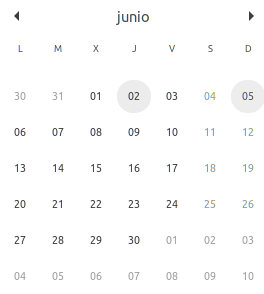
\includegraphics[width=0.3\textwidth]{img/calendario-2.png}
    \caption{Calendario de la nueva fecha de finalización del proyecto. [Elaboración propia]}
    \label{fig:calendario-2}
\end{figure}

\begin{table}[]
	\begin{center}
		\begin{tabular}{| c | l | c |}
			\hline
			\textbf{Código} & \textbf{Tarea}                                                 & \textbf{Tiempo} \\ \hline
			\textbf{T1}     & \textbf{Documentación}                                         & \textbf{180 h}  \\ \hline
			T1.1            & Contexto y Alcance                                             & 20 h            \\
			T1.2            & Planificación Temporal                                         & 10 h            \\
			T1.3            & Presupuesto y sostenibilidad                                   & 10 h            \\
			T1.4            & Memoria final                                                  & 70 h            \\
			T1.5            & Presentación                                                   & 10 h            \\
			T1.6            & Reuniones                                                      & 6 h             \\
			T1.7            & Documentación del entorno                                      & 40 h            \\
			T1.8            & Documentación del código                                       & 14 h            \\
			\hline
			\textbf{T2}     & \textbf{Creación del entorno}                                  & \textbf{320 h}  \\ \hline
			T2.1            & Búsqueda y valoración del estado del arte                      & 60 h            \\ \hline
			T2.1.1          & Definición de las métricas usadas para valorar los entornos    & 5 h             \\
			T2.1.2          & Búsqueda y valoración de entornos funcionales                  & 25 h            \\
			T2.1.3          & Búsqueda y valoración de entornos no funcionales               & 25 h            \\
			T2.1.4          & Valoración de los entornos encontrados y selección final       & 5 h             \\ \hline
			T2.2            & Aprendizaje del entorno                                        & 50 h            \\ \hline
			T2.2.1          & Búsqueda de los módulos a modificar                            & 5 h             \\
			T2.2.2          & Aprendizaje del lenguaje de programación Lua                   & 30 h            \\
			T2.2.3          & Aprendizaje de la API de PettingZoo                            & 15 h            \\ \hline
			T2.3            & Diseño de las nuevas características                           & 60 h            \\ \hline
			T2.3.1          & Diseño del sistema de visualización del entorno                & 15 h            \\
			T2.3.2          & Diseño del sistema de comunicación entre procesos              & 25 h            \\
			T2.3.2          & Diseño del sistema de acciones de la IA                        & 20 h            \\ \hline
			T2.4            & Implementación de las nuevas características                   & 100 h            \\ \hline
			T2.4.1          & Solución de problemas en la implementación                     & 40 h            \\\hline

			T2.5            & Testing y creación de los agentes                              & 50 h            \\ \hline
			T2.5.1          & Configuración del entorno para el entrenamiento de los agentes & 10 h            \\
			\hline
			\textbf{Total}  &                                                                & \textbf{500 h}  \\
			\hline
		\end{tabular}
		\caption{Resumen final detallado de las tareas que forman el proyecto [Elaboración propia]}
		\label{tab:planificacion-2}
	\end{center}
\end{table}



